\documentclass{homeworg}
\usepackage{enumitem}
\usepackage{listings}
\usepackage{color} %red, green, blue, yellow, cyan, magenta, black, white
\definecolor{mygreen}{RGB}{28,172,0} % color values Red, Green, Blue
\definecolor{mylilas}{RGB}{170,55,241}
\usepackage{xcolor,cancel}
% --------------- GRAPHIC PACKAGES ----------------------------
\usepackage{graphicx}
\graphicspath{{./images/}}
\usepackage{wrapfig}
% --------------- HCANCEL COMMAND -----------------------------
\newcommand\hcancel[2][black]{\setbox0=\hbox{$#2$}%
\rlap{\raisebox{.45\ht0}{\textcolor{#1}{\rule{\wd0}{1pt}}}}#2}

% --------------- TRANSPOSE COMMAND -----------------------------
\newcommand{\transpose}[1]{\ensuremath{#1^{\scriptscriptstyle T}}}


\begin{document}

% --------------- MATLAB Code settings -----------------------
\lstset{language=Matlab,%
    %basicstyle=\color{red},
    breaklines=true,%
    morekeywords={matlab2tikz},
    keywordstyle=\color{blue},%
    morekeywords=[2]{1}, keywordstyle=[2]{\color{black}},
    identifierstyle=\color{black},%
    stringstyle=\color{mylilas},
    commentstyle=\color{mygreen},%
    showstringspaces=false,%without this there will be a symbol in the places where there is a space
    numbers=left,%
    numberstyle={\tiny \color{black}},% size of the numbers
    numbersep=9pt, % this defines how far the numbers are from the text
    emph=[1]{for,end,break},emphstyle=[1]\color{red}, %some words to emphasise
    %emph=[2]{word1,word2}, emphstyle=[2]{style},
}

% --------------- Title -------------------------------------
%\maketitle
\begin{center}
\textbf{EE 5323 - HW07}\\
\end{center}

\noindent
Bardia Mojra\\
1000766739\\
\today\\
HW07 -- Lyapunov Control Design, Feedback Linearization\\
EE 5323 -- Nonlinear Systems\\
Dr. Frank Lewis

\exercise
\noindent
\textbf{Control Desing}\\
Consider the following system,
\begin{equation*}
  \begin{array}{lcl}
    \dot{x}_1 = x_2 \sin(x_1)\\
    \dot{x}_2 = x_1 x_2 + u \\
  \end{array}
\end{equation*}
Select Lyapunov function candidate
\begin{equation*}
V(x) = \frac{1}{2} (x_1^2  + x_2^2)
\end{equation*}
Use Lyapunov to design a controller u(x) to make system SISL.



We used a quadratic Lyapunov Function to show this system is locally SISL.
And we found the region within which \(\dot{V} \leq 0\).
Use LaSalle’s extension to verify that the system is AS. Find the
equilibrium point.\\
\noindent
\textbf{Answer} \\
1.a) Lyapunov function candidate: \( V(x_1, x_2) = \frac{1}{2} (x_1^2 + x_2^2) > 0\)
\begin{equation*}
\dot{V} = \frac{\partial V^\top}{\partial x} \dot{x} =
\begin{bmatrix}
\frac{\partial V}{\partial x_1} & \frac{\partial V}{\partial x_2}
\end{bmatrix}
\begin{bmatrix}
\dot{x}_1 \\
\dot{x}_2
\end{bmatrix}
=
\begin{bmatrix}
  x_1 & x_2
  \end{bmatrix}
  \begin{bmatrix}
  \dot{x}_1 \\
  \dot{x}_2
  \end{bmatrix}
  \Rightarrow
\end{equation*}
\begin{equation*}
\dot{V} =
  x_1 \dot{x}_1 + x_2 \dot{x}_2
\end{equation*}
Now we plug in system dynamics to check stability,
\begin{equation*}
  \dot{V} = x_1 (x_2 + x_1 (x_1^2 -2)) + x_2(-x_1) \Rightarrow
\end{equation*}
\begin{equation*}
  \dot{V} = \hcancel[red]{x_1 x_2} - x_1^2(x_1^2 -2) - \hcancel[red]{x_1 x_2}
\end{equation*}
\begin{equation*}
  \dot{V} = - x_1^2(x_1^2 -2) \leq 0
\end{equation*}
Thus, the system is \emph{asymptotically stable} (AS) and it is bound by a region
with radius of \(\sqrt{2}\). Moreover, we know \(\dot{x} \rightarrow 0\); thus,
per LaSalle’s extension, \(\ddot{x} \rightarrow 0\) must hold true and that makes
\(x_1,x_2 \rightarrow 0\) at \(t= \infty\). We proceed with plugging in the
resulting \(x_1\) in the system dynamics equation.
\begin{equation*}
  \dot{V} = - x_1^2(x_1^2 -2) \leq 0 \Rightarrow \dot{V} \rightarrow 0,~x_1~|~x_{1}^{2}  = 2; \Rightarrow x_1 = \{0, \pm \sqrt{2} \},~x_2 = 0
\end{equation*}
Where e.p.s would be \((-\sqrt{2},~0),~(0,~0),~(+\sqrt{2},~0)\).
\newpage
1.b) Simulation:
\begin{figure}[!htb]
  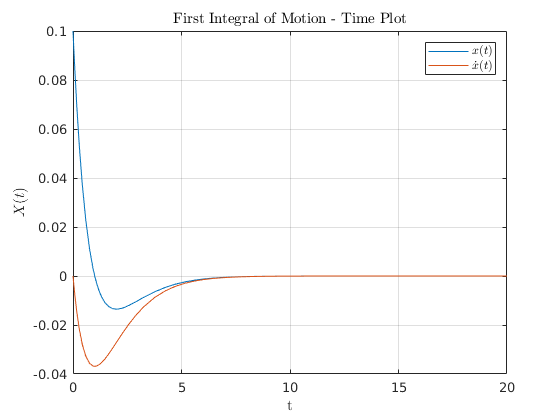
\includegraphics[width=.5\textwidth]{fig01.png}
  \centering
  \caption{}
\end{figure}
\begin{figure}[!htb]
  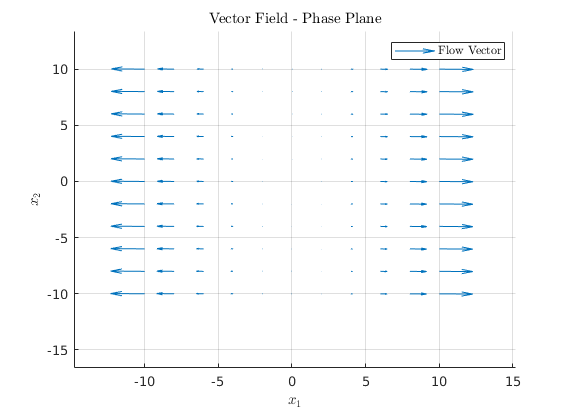
\includegraphics[width=.5\textwidth]{fig02.png}
  \centering
  \caption{}
\end{figure}
\begin{figure}[!htb]
  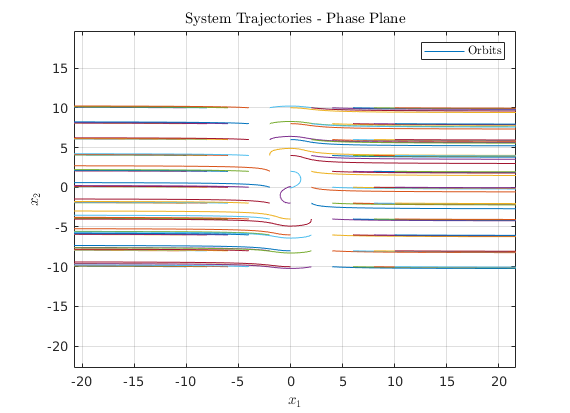
\includegraphics[width=.5\textwidth]{fig03.png}
  \centering
  \caption{}
\end{figure}

\clearpage
\noindent
\textbf{Matlab Code}
\lstinputlisting{../src/q01_main.m}
\lstinputlisting{../src/q01_sys.m}

\exercise
\noindent
\textbf{Limit Cycles}\\
Consider the following system,
\begin{equation*}
  \begin{cases}
    \dot{x} = 4 x^2 y - f_1 (x) \left( x^2 + 2 y^2 -4  \right)\\
    \dot{y} = 2 x^3 - f_2 (y) \left( x^2 + 2 y^2 -4  \right)\\
  \end{cases}
\end{equation*}
where the continuous functions \(f_1 (x)\), \(f_2 (y)\) have the same sign as
their argument. Show that the system tends towards a limit cycle independent
of the explicit expressions of \(f_1 (x)\), \(f_2 (y)\).
\noindent
\textbf{Answer} \\
2.a) Weird Lyapunov function candidate:\(V(x, y)= \frac{1}{2}(x^2 + 2y^2 -4)^2 > 0\)
\begin{equation*}
\dot{V} = \frac{1}{2} 2 (x^2 + 2y^2 -4)(2x \dot{x} + 4y \dot{y})
\end{equation*}
Now we plug in system dynamics to check stability,
\begin{equation*}
  \dot{V}=(x^2+2y^2-4)\left[2x\left(4x^2y-f_1(x)(x^2+2y^2-4)\right)+4y\left(2x^3-f_2(y)(x^2+2y^2-4)\right)\right]\Rightarrow
\end{equation*}
\begin{equation*}
  \dot{V}=(x^2+2y^2-4)^2
  \left[2x\left(4x^2y-f_1(x)\right)+4y\left(2x^3-f_2(y)\right)\right]\Rightarrow
\end{equation*}
\begin{equation*}
  \dot{V}=(x^2+2y^2-4)^2
  \left[
    16x^3y-2xf_1(x)-4yf_2(y)
    \right]\Rightarrow
\end{equation*}
Thus, \(\dot{V} < 0\) unless \( (x^2+2y^2-4) = 0 \) which makes \( \lim_{t\to \infty} \liminf{  \dot{V}} \rightarrow 0\). The invariant set forms a \emph{Stable
Limit Cycle} about \((x^2+2y^2-4)=0\).\\

\noindent
2.b) Simulation:
\begin{figure}[!htb]
  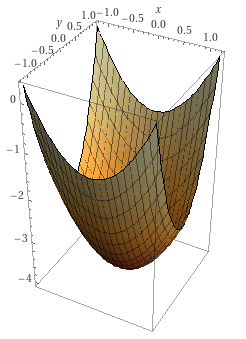
\includegraphics[width=.3\textwidth]{fig04.png}
  \centering
  \caption{3D Plot}
\end{figure}
\begin{figure}[!htb]
  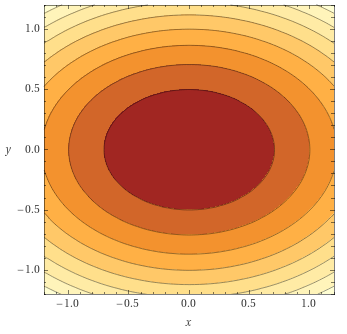
\includegraphics[width=.3\textwidth]{fig05.png}
  \centering
  \caption{Contour Plot}
\end{figure}


\exercise % 3
\noindent
\textbf{UUB of System with Disturbance}\\
Consider the system on S\&L p. 66 with a disturbance d,
\begin{equation*}
  \dot{x} + C(x) + d = 0
\end{equation*}
Assume that \(xC(x) > a x^2 \) with \( a > 0\) a known positive constant.\\
a. Assume that d is unknown but is bounded by \(\|d\| < D \) with D a known
positive constant. Prove that the system is UUB and find the bound on \(x(t)\).\\
b. Assume that d is unknown but is bounded by \(\|d\| < D\|x\| \) with D a
known positive constant. Prove that the system is UUB and find the bound
on \(x(t)\).\\
\noindent
\textbf{Answer} \\
1.a) We proceed with selecting a Lyapunov function candidate and normalizing its
first derivative.\\
\begin{equation*}
  \dot{x} + C(x) + d = 0 \Rightarrow \dot{x} = - C(x) - d \\
\end{equation*}
\begin{equation*}
  V=\frac{1}{2}x^2\Rightarrow \dot{V} = x\dot{x} \Rightarrow \dot{V} =-xC(x)-xd \\
\end{equation*}
per Cauchy-Schwarz \(\mathbb{R}^2\):
\begin{equation*}
  \left<x,y\right>^{1/2} = \| \transpose{x}y\| \leq \|x\| \cdot \|y\|~; \textit{ thus, } \|Ax\| \leq \|A\| \cdot \|x\|
\end{equation*}
\begin{equation*}
  \dot{V} = -\|x\|C(x)-\|xd\| \leq  -\|x\|C(x)-\|x\| \|d\| \\
\end{equation*}
\begin{equation*}
  \dot{V} \leq  -\|x\|C(x)-\|x\| \|d\| = -\|x\|(C(x)+\|d\|) ;\\
\end{equation*}
Since xC(x) >> 0, x and C(x) must have the same sign, thus \(\dot{V} \leq 0 \) when,
\begin{equation*}
  C(x)+\|d\| > 0 \Rightarrow C(x) > -\|d\| ; \|d\| < D \Rightarrow - D < C(x)< D
\end{equation*}
Thus, C(x) term is bounded by \(\pm D\).\\

1.b) We continue from the last step.
\begin{equation*}
  \dot{V} \leq  -\|x\|(C(x)+\|d\|), \\
\end{equation*}
So \(\dot{V} \leq 0 \) when, \(C(x)+\|d\| >0\) where \(\|d\| < D\|x\| \)
\begin{equation*}
  C(x) > - \|d\| \Rightarrow -D\|x\| < C(x)\|x\| < +D\|x\| \Rightarrow
\end{equation*}
\begin{equation*}
  -D < \frac{C(x)}{\|x\|} < +D
\end{equation*}

\exercise
\noindent
\textbf{Lyapunov Equation}\\
Use Lyapunov Equation to check the stability of the linear systems.

a. \( \dot{x} = Ax = \begin{bmatrix}
  0 & 1\\
  -6 & -5\\
\end{bmatrix} x \)

b. \( \dot{x} = Ax = \begin{bmatrix}
  -7 & 4\\
  -7 & 3\\
\end{bmatrix} x \)

c. \( \dot{x} = Ax = \begin{bmatrix}
   0 & 1\\
  -4 & 0\\
\end{bmatrix} x \)

\noindent
\textbf{Answer} \\
a.) \(\transpose{A}P+PA=-Q \)
\begin{equation*}
\begin{bmatrix}
    a_1 & a_3\\
    a_2 & a_4\\
\end{bmatrix}
\begin{bmatrix}
  p_1 & p_2\\
  p_2 & p_3\\
\end{bmatrix} +
\begin{bmatrix}
p_1 & p_2\\
p_2 & p_3\\
\end{bmatrix}
\begin{bmatrix}
  a_1 & a_2\\
  a_3 & a_4\\
\end{bmatrix} = -Q
\end{equation*}
\begin{equation*}
\begin{bmatrix}
  a_1 p_1 + a_3 p_3 & a_1 p_2 + a_3 p_3 \\
  a_2 p_1 + a_4 p_2 & a_2 p_2 + a_4 p_3 \\
\end{bmatrix}
\begin{bmatrix}
  a_1 p_1 + a_3 p_2 & a_2 p_1 + a_4 p_2 \\
  a_1 p_2 + a_3 p_3 & a_2 p_2 + a_4 p_3 \\
\end{bmatrix} = -Q
\end{equation*}
\begin{equation*}
  \begin{bmatrix}
    a_1 p_1 + a_3 p_3 + a_1 p_1 + a_3 p_2 & a_1 p_2 + a_3 p_3 + a_2 p_1 + a_4 p_2\\
    a_2 p_1 + a_4 p_2 + a_1 p_2 + a_3 p_3 & a_2 p_2 + a_4 p_3 + a_2 p_2 + a_4 p_3\\
  \end{bmatrix} = -Q
\end{equation*}
\begin{equation*}
\begin{bmatrix}
    -6 p_3 + -6 p_2 & -6 p_3 + p_1 + -5 p_2\\
    p_1 + -5 p_2 + -6 p_3 & p_2 + -5 p_3 + p_2 + -5 p_3\\
\end{bmatrix} =
\begin{bmatrix}
  0 & 0\\
  0 & -1\\
\end{bmatrix} \Rightarrow
P = \begin{bmatrix}
  .0167 & 0\\
  0 & .1\\
\end{bmatrix}
\end{equation*}\\
where \(m_{11}= .0167, m_{22}= ~.00167\) so it is positive definite.\\

b.) \(\transpose{A}P+PA=-Q \)
\begin{equation*}
\begin{bmatrix}
  -7 & -7\\
  4 & 3\\
\end{bmatrix}
\begin{bmatrix}
  p_1 & p_2\\
  p_2 & p_3\\
\end{bmatrix} +
\begin{bmatrix}
p_1 & p_2\\
p_2 & p_3\\
\end{bmatrix}
\begin{bmatrix}
  -7 & 4\\
  -7 & 3\\
\end{bmatrix} = -Q
\end{equation*}
\begin{equation*}
\begin{bmatrix}
    -7 p_1 + -7 p_3 + -7 p_1 + -7 p_2 & -7 p_2 + -7 p_3 + 4 p_1 + 3 p_2\\
    4 p_1 + 3 p_2 + -7 p_2 + -7 p_3 & 4 p_2 + 3 p_3 + 4 p_2 + 3 p_3\\
\end{bmatrix} =
\begin{bmatrix}
  0 & 0\\
  0 & -1\\
\end{bmatrix} \Rightarrow
P = \begin{bmatrix}
  .2857 & .5\\
  .5 & 1\\
\end{bmatrix}
\end{equation*}\\
where \(m_{11}= .2857, m_{22}= ~.0357\) so it is positive definite.\\

c.) \(\transpose{A}P+PA=-Q \)
\begin{equation*}
\begin{bmatrix}
  0 & -4\\
  1 & 0\\
\end{bmatrix}
\begin{bmatrix}
  p_1 & p_2\\
  p_2 & p_3\\
\end{bmatrix} +
\begin{bmatrix}
p_1 & p_2\\
p_2 & p_3\\
\end{bmatrix}
\begin{bmatrix}
  0 & 1\\
  -4 & 0\\
\end{bmatrix} = -Q
\end{equation*}
\begin{equation*}
\begin{bmatrix}
  -4 p_3 + -4 p_2 & -4 p_3 + 1 p_1 \\
  1 p_1 + -4 p_3 & 1 p_2 + 1 p_2 \\
\end{bmatrix} =
\begin{bmatrix}
  0 & 1\\
  -1 & 0\\
\end{bmatrix} \Rightarrow
P = \text{undetermined}
\end{equation*}
The system is unstable and does not have a unique solution.\\
\end{document}
